\chapter{流体静力学}\label{ch:b1:fluid-statics}

一艘位于三百米深处的潜艇，其船体每平方米承受的
压力，相当于一辆满载卡车的重量。
水坝拦住湖水，墙体下厚上薄，
其原因与湖的长短毫无关系。一艘十万吨的轮船
能够浮在水面，是因为它排开了十万吨的水；
当它从海里驶入河中时，船身会下沉一掌宽的深度。
上述每一种现象都源于同一个关系
——静止流体中压强沿竖直向下以 $\rho g$ 的变化率增加——
本章推导该关系，并将其应用于液体与大气，
由此进一步导出器壁所受的力以及阿基米德定律。

\begin{omfigure}
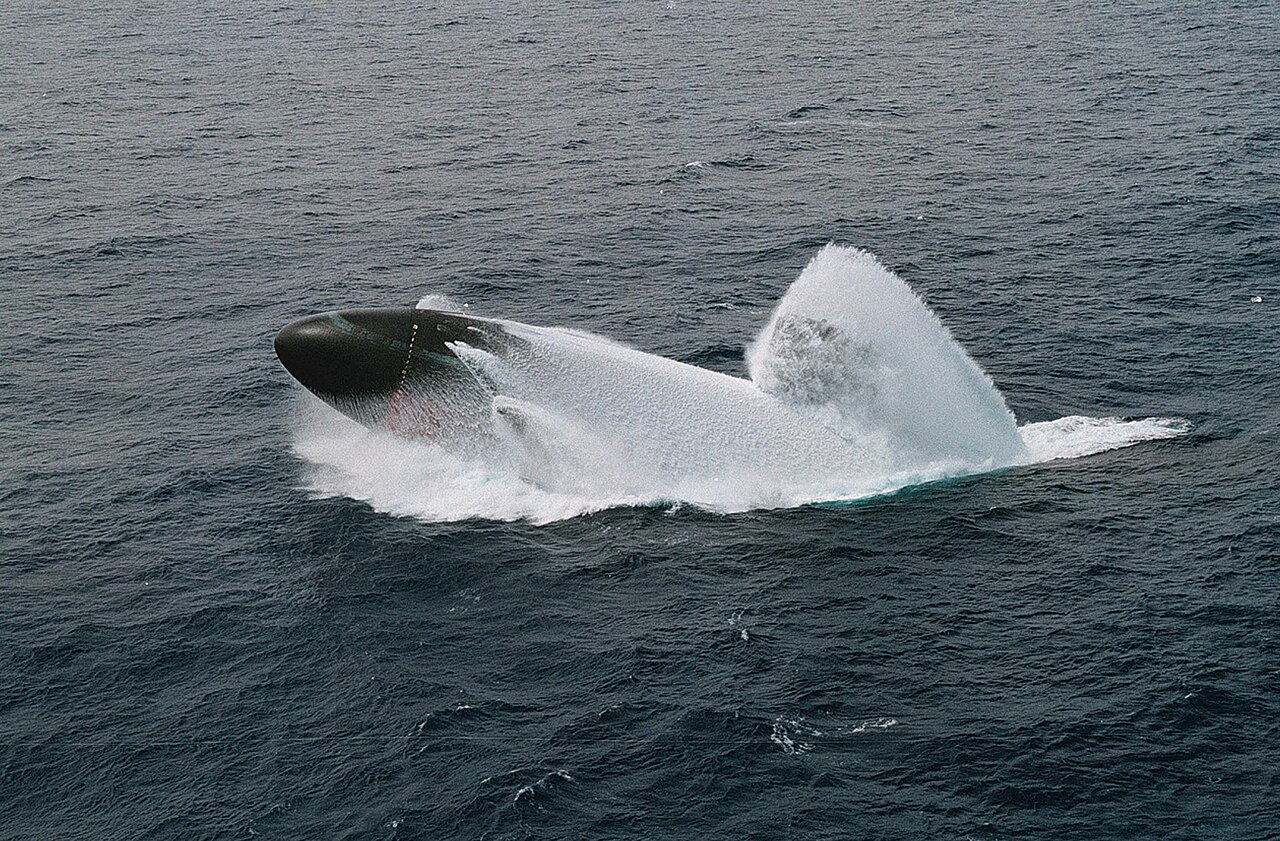
\includegraphics[width=0.60\linewidth]{images/book3/submarine-surfacing.jpg}

{\small 美国海军紧急上浮演练中的潜艇：压载水舱排空后，它比所排开的水更轻，于是上浮——阿基米德定理在 \qty{7000}{t} 时的体现。}
\end{omfigure}

\section{静止流体中的压强}

\begin{proposition}[压强的各向同性]\label{prop:b1:fluid-statics:isotropy}
\index{压强!在流体中}
在静止流体中，流体作用于一小块曲面面元上的力，
设面元 $\dd S$ 位于点 $M$ 处，则该力为 $\dd\vect F = P(M)\,\dd S\,\vect n$，法向于
曲面并指向该曲面，压强 $P(M)$ 随点而变，
但\emph{不}随曲面的取向而变。
\end{proposition}

\begin{proof}[部分证明]
静止流体不传递切向力（否则它将流动）：
因此作用力必沿法向。考虑 $M$ 处一个微小的三棱柱形流体，
其各面取向不同：它在各面上的压力及自身重力作用下处于平衡，
重力随体积变化，即与线度的三次方成正比，
压力则与面积成正比，即与线度的二次方成正比，
因此对于足够小的棱柱，只有压力起作用，
其在各方向上的平衡要求各面上的 $P$ 相同。
\end{proof}

\begin{theorem}[流体静力学基本关系]\label{thm:b1:fluid-statics:fundamental}
\index{流体静力学基本关系}
在匀强重力场 $\vect g = -g\vect e_z$ 中静止的流体（
$z$ 轴竖直向上），压强仅依赖于 $z$，并且
\[
\frac{\dd P}{\dd z} = -\rho g ,
\]
$\rho$ 为该高度处流体的密度。压强向下增大；
压强相等的面（\emph{等压面}）是水平的，
液体的自由表面也是水平的。
\end{theorem}

\begin{proof}
取面积为 $S$、位于 $z$ 与 $z + \dd z$ 之间的水平薄层流体：
它下方受 $P(z)S$ 的压力向上推，上方受 $P(z + \dd z)S$ 的压力向下压，
并受重力 $\rho gS\,\dd z$ 向下拉。静止时有：
$P(z)S - P(z + \dd z)S - \rho gS\,\dd z = 0$。水平薄层流体
在水平方向上不受重力分量，故 $P$ 在水平方向上是均匀的。
\end{proof}

\begin{omfigure}
\begin{tikzpicture}[font=\small, x=1cm, y=1cm]
  \fill[omDef!10] (-2.4,-1.8) rectangle (2.4,1.8);
  \draw[thick, fill=omDef!30] (-1.2,-0.25) rectangle (1.2,0.25);
  \draw[-Stealth, omThm, very thick] (0,-1.3) -- (0,-0.3) node[pos=0.0, below] {$P(z)\,S$};
  \draw[-Stealth, omThm, very thick] (0,1.3) -- (0,0.3) node[pos=0.0, above] {$P(z + \dd z)\,S$};
  \draw[-Stealth, omProp, very thick] (0.9,0) -- (0.9,-0.9) node[right] {$\rho gS\,\dd z$};
  \draw[Stealth-Stealth] (-1.5,-0.25) -- (-1.5,0.25) node[midway, left] {$\dd z$};
  \draw[-Stealth] (2.8,-1.5) -- (2.8,1.5) node[above] {$z$};
  \node[font=\footnotesize] at (0,-2.1) {$P(z) - P(z + \dd z) = \rho g\,\dd z$};
\end{tikzpicture}\qquad
\begin{tikzpicture}[font=\small, x=1cm, y=1cm]
  % communicating vessels
  \fill[omDef!25] (0,0) rectangle (0.8,2.4); \fill[omDef!25] (0,0) rectangle (4.2,0.6); \fill[omDef!25] (1.8,0) rectangle (2.4,2.4); \fill[omDef!25] (3.4,0) rectangle (4.2,2.4);
  \draw[thick] (0,3.2) -- (0,0) -- (4.2,0) -- (4.2,3.2); \draw[thick] (0.8,3.2) -- (0.8,0.6) -- (1.8,0.6) -- (1.8,3.2); \draw[thick] (2.4,3.2) -- (2.4,0.6) -- (3.4,0.6) -- (3.4,3.2);
  \draw[omDef, thick] (0,2.4) -- (0.8,2.4); \draw[omDef, thick] (1.8,2.4) -- (2.4,2.4); \draw[omDef, thick] (3.4,2.4) -- (4.2,2.4);
  \draw[dashed, omThm] (-0.3,2.4) -- (4.5,2.4); \node[omThm, right] at (4.5,2.4) {同一水平面};
  \node[font=\footnotesize] at (2.1,-0.4) {水平线上 $P$ 处处相同};
\end{tikzpicture}

{\small 左：水平流体薄层的平衡——下方压强须比上方压强大，
其差值等于该薄层单位面积上的重力。右：连通容器——同一水平线上
各点在连通液体中压强相同，
因此无论容器形状如何，各容器中的自由表面
都处于同一高度。}
\end{omfigure}

\begin{corollary}[不可压缩流体]\label{cor:b1:fluid-statics:incompressible}
\index{静压强}
在密度为 $\rho$ 的均匀液体中，比某点低 $h$ 深处的压强
（该点压强为 $P_0$）为
\[
P = P_0 + \rho gh .
\]
水中每增加 \qty{10}{m} 深度，压强增加 \qty{1}{bar}。连通液体中
处于同一高度的两点压强相等；连通容器的自由表面
处于同一高度；密闭液体中任一处施加的压强，
将不减小地传递到液体的每一点（帕斯卡原理）。
%
\end{corollary}

\begin{proof}
对 $\dd P/\dd z = -\rho g$ 积分，其中 $\rho$ 为常数；其余部分由
等压面的水平性与同一高度处 $P$ 的唯一性得到。
\end{proof}

\begin{example}[压强计与液压机]\label{ex:b1:fluid-statics:manometer}
\index{压强计}\index{液压机}
装汞的 U 形管（$\rho = \qty{13600}{kg/m^3}$），两管液柱高度差为
$h = \qty{760}{mm}$ 时，即测得压强差 $\rho gh = \qty{1.013e5}{Pa}$
——相当于大气压，它能托起 \qty{10.3}{m} 高的水柱。
液压机中，力 $F_1$ 作用于面积为 $S_1$ 的活塞上，使
整个液体的压强增加 $F_1/S_1$；在大活塞 $S_2$ 上，
可得 $F_2 = F_1S_2/S_1$——面积增大五十倍，力也增大五十倍，
代价是行程减小到原来的五十分之一（能量守恒：$F_1d_1 = F_2d_2$）。
\end{example}

\section{大气层}

\begin{proposition}[等温大气]\label{prop:b1:fluid-statics:atmosphere}
\index{气压公式}\index{标高}
设摩尔质量为 $M$ 的理想气体，温度 $T$ 处处均匀，
处于均匀重力场中，
\[
P(z) = P_0\,\eu^{-z/H}, \qquad H = \frac{RT}{Mg} ,
\]
\emph{标高}：空气约为 \qty{8}{km}；
每升高 $H\ln2 \approx \qty{5.5}{km}$，压强减半。
\end{proposition}

\begin{proof}
由状态方程 $\rho = PM/RT$，可得 $\dd P/\dd z = -(Mg/RT)P$，
这是一阶线性方程，$P = P_0\eu^{-Mgz/RT}$。
\end{proof}

\begin{example}[稀薄空气]\label{ex:b1:fluid-statics:altitude}
取 $T = \qty{260}{K}$（低层大气的平均值），$H =
\qty{7.6}{km}$：$P = 0.52P_0$（\qty{5000}{m} 处），$0.31P_0$（珠穆朗玛峰
峰顶）——与实测值 $0.54$ 和 $0.33$ 接近；真实大气
随高度降温，这一点在本科二年级分册中予以考虑。
模型还能说明海洋为何不同：水的密度是空气的八百倍，
且几乎不可压缩，因此其压强线性增长，每十米增加一巴，
没有标高。
\end{example}

\begin{omfigure}
\begin{tikzpicture}
\begin{axis}[omaxis, axis x line=bottom, axis y line=left, width=8cm, height=5.4cm, xlabel={$z$ (\unit{km})}, ylabel={$P/P_0$},
    xlabel style={at={(axis description cs:0.5,-0.12)}, anchor=north},
    xmin=0, xmax=30, ymin=0, ymax=1.1, xtick={5.5,10,20,30}, xticklabels={$5.5$,$10$,$20$,$30$}, ytick={0.5,1}]
  \addplot[omDef, thick, domain=0:30, samples=100] {exp(-x/7.6)};
  \draw[dashed, omExo] (axis cs:0,0.5) -- (axis cs:5.3,0.5) -- (axis cs:5.3,0);
  \node[omDef, font=\footnotesize] at (axis cs:16,0.45) {$P_0\eu^{-z/H}$, $H = \qty{7.6}{km}$};
\end{axis}
\end{tikzpicture}

{\small 等温大气中，压强（及密度）随高度按指数规律下降，
每升高 \qty{5.5}{km} 压强减半。十分之九的空气
位于 \qty{17}{km} 以下。}
\end{omfigure}

\section{器壁上的力}

\begin{proposition}[竖直墙壁上的力]\label{prop:b1:fluid-statics:wall}
\index{压力中心}
深度为 $h$ 的液体作用于宽为 $L$ 的竖直矩形墙壁上
（大气压强作用于两侧并相互抵消），给出
水平方向的力
\[
F = \tfrac12\rho gh^2L ,
\]
它等效于一个作用在\emph{压力中心}上的力，
位于深度 $2h/3$ 处——合力作用点偏低，此处压强
最大。
\end{proposition}

\begin{proof}
深度为 $x$ 处的表压为 $\rho gx$；
在高为 $\dd x$ 的条带上，受力为 $\rho gxL\,\dd x$；
从 $0$ 到 $h$ 积分。其对液面线的力矩为 $\int_0^h\rho gx^2L\,\dd x = \tfrac13\rho gh^3L$；
除以 $F$ 得力臂 $2h/3$。
\end{proof}

\begin{omfigure}
\begin{tikzpicture}[font=\small, x=1cm, y=1cm]
  \fill[omDef!20] (-3.6,0) rectangle (0,2.8);
  \draw[thick] (-3.8,2.8) -- (0,2.8); \draw[omDef, thick] (-3.6,2.8) -- (0,2.8);
  \draw[thick, fill=omExo!40] (0,0) -- (0,3.2) -- (1.0,3.2) -- (1.8,0) -- cycle;
  \draw[thick] (-3.8,0) -- (2.6,0);
  \foreach \y/\l in {2.5/0.15, 2.0/0.4, 1.5/0.65, 1.0/0.9, 0.5/1.15, 0.1/1.35} {\draw[-Stealth, omThm] (-\l,\y) -- (0,\y);}
  \draw[omThm, dashed] (0,2.8) -- (-1.4,0);
  \draw[-Stealth, omThm, very thick] (-2.6,0.93) -- (-0.05,0.93) node[pos=0.0, left] {$F = \tfrac12\rho gh^2L$};
  \draw[Stealth-Stealth] (2.2,2.8) -- (2.2,0.93) node[midway, right] {$\tfrac23 h$};
  \draw[Stealth-Stealth] (-3.2,2.8) -- (-3.2,0) node[midway, left] {$h$};
\end{tikzpicture}

{\small 坝面上的压强随深度线性增加（箭头所示），因此
合力作用于深度的三分之二处：墙体底部须最厚。
作用力只取决于 $h$ 与 $L$，
与背后蓄水多少无关。}
\end{omfigure}

\begin{example}[水坝]\label{ex:b1:fluid-statics:dam}
$h = \qty{20}{m}$，$L = \qty{100}{m}$：$F = \tfrac12 \times 1000 \times 9.81 \times
400 \times 100 = \qty{2.0e8}{N}$——约两万吨，作用于
液面以下 \qty{13}{m} 处，无论背后的湖泊是池塘还是
峡湾，作用力都相同：这就是\emph{静水佯谬}。
\end{example}

\section{阿基米德定理}

\begin{theorem}[阿基米德]\label{thm:b1:fluid-statics:archimedes}
\index{阿基米德定理}\index{浮力}\index{浮心}
浸没在静止流体中的物体，受到压力的合力
——即\emph{浮力}——与其所排开流体的重力
大小相等、方向相反，
\[
\vect\Pi = -\rho_{\text{流体}}V_{\text{浸没}}\,\vect g ,
\]
作用于所排开流体的质心（\emph{浮心}
）。
\end{theorem}

\begin{proof}
物体表面上的压力只取决于该表面的形状
以及外部流体。设想以体积相同的静止流体
取代物体，该流体在重力及同样的压力作用下
处于平衡，因此压力的合力与其重力平衡，
合力为 $-\rho V\vect g$，作用于其
质心。去掉这一思想实验后，压力
保持不变。
\end{proof}

\begin{corollary}[漂浮]\label{cor:b1:fluid-statics:floating}
\index{漂浮}
密度为 $\rho_b$ 的物体漂浮于密度为 $\rho_f > \rho_b$
的流体中，浸入部分占其体积的比例为 $\rho_b/\rho_f$；若 $\rho_b >
\rho_f$，则物体下沉，视重为 $(\rho_b - \rho_f)Vg$。
\end{corollary}

\begin{proof}
重力 $\rho_bVg$ 等于浮力 $\rho_fV_{\text{浸没}}g$。
\end{proof}

\begin{omfigure}
\begin{tikzpicture}[font=\small, x=1cm, y=1cm]
  \fill[omDef!15] (-3.6,-2.2) rectangle (3.6,0);
  \draw[omDef, thick] (-3.6,0) -- (3.6,0);
  % iceberg-like block: rectangle 2 x 1.6, 90% immersed
  \draw[thick, fill=white] (-1.0,-1.44) rectangle (1.0,0.16);
  \fill (0,-0.64) circle (1.5pt) node[right] {$G$};
  \fill[omDef] (0,-0.72) circle (1.5pt) node[left] {$C$};
  \draw[-Stealth, omThm, very thick] (0,-0.64) -- (0,-1.9) node[below] {$\rho_bVg$};
  \draw[-Stealth, omDef, very thick] (0,-0.72) -- (0,0.55) node[above] {$\rho_fV_{\text{浸没}}g$};
  \node[font=\footnotesize] at (2.4,-1.2) {$\dfrac{V_{\text{浸没}}}{V} = \dfrac{\rho_b}{\rho_f}$};
\end{tikzpicture}

{\small 漂浮物体：其重力作用于质心 $G$，
与作用于浮心 $C$ 的浮力平衡（浮心
即浸没体积的中心）。冰（$\rho = \qty{917}{kg/m^3}$）置于海水
（$\qty{1025}{kg/m^3}$）中：$89\%$ 位于水面以下。}
\end{omfigure}

\begin{example}[三个浮力的例子]\label{ex:b1:fluid-statics:buoy}
密度计是一根带配重的细管，下沉至排开的液体重量恰好等于
其自身重量；液体密度越大，下沉越少——密度值直接标在管柄上。
一只 \qty{2800}{m^3} 的热空气气球，温度为 \qty{373}{K}，排开
\qty{3.4}{t} 的冷空气，其内热空气重 \qty{2.6}{t}，净升力为
\qty{0.7}{t}（见\cref{pb:b1:kinetic-theory:1}）。一艘 \qty{100000}{t} 的船
排开 \qty{97600}{m^3} 的海水；在淡水（$\qty{1000}{kg/m^3}$）中
它须多排开 $2.5\%$ 的水，下沉得更深——此即船身上的
普利姆索尔线。
\end{example}

\begin{remark}[稳定性]\label{rem:b1:fluid-statics:stability}
\index{稳心}
漂浮物体受微小倾斜后，若浮力
作用于新浸没体积的移动中心并产生复原力矩，则物体可复位——这发生于
\emph{稳心}（即浮力作用线与物体轴线的
交点）位于
$G$ 之上时。船底低处的压舱物降低 $G$，使船稳定；
头重脚轻的小船会倾覆。
\end{remark}

\section{练习}

\begin{exercise}[$\star$]\label{exo:b1:fluid-statics:1}
求海水中 \qty{10}{m}、\qty{100}{m} 与 \qty{1}{km} 处的绝对压强
（$\rho = \qty{1025}{kg/m^3}$）；求面积为 \qty{1.0}{m^2}
的舷窗在 \qty{300}{m} 深处所受的压力。
\end{exercise}

\begin{exercise}[$\star$]\label{exo:b1:fluid-statics:2}
求与 \qty{1.013e5}{Pa} 相平衡的水银柱高度，以及
水柱高度。说明抽水泵为何不能把水提升超过约 \qty{10}{m}。
\end{exercise}

\begin{exercise}[$\star$]\label{exo:b1:fluid-statics:3}
一液压千斤顶：在面积为 \qty{2.0}{cm^2} 的活塞上施力 \qty{100}{N}，负载
位于面积为 \qty{200}{cm^2} 的活塞上；若小活塞移动 \qty{20}{cm}，
求两活塞各自移动的距离。
\end{exercise}

\begin{exercise}[$\star$]\label{exo:b1:fluid-statics:4}
U 形管中盛有水，向一侧管中注入油（$\rho = \qty{850}{kg/m^3}$），
在该侧形成 \qty{12}{cm} 高的油柱。求两
自由液面之间的高度差。
\end{exercise}

\begin{exercise}[$\star\star$]\label{exo:b1:fluid-statics:5}
求 \qty{273}{K} 时大气的标高、\qty{5000}{m} 处的压强
及 \qty{8848}{m} 处的压强，以及满足 $P = P_0/2$ 的高度。将结果
与在\cref{ch:b1:kinetic-theory}中给出的数值进行比较。
\end{exercise}

\begin{exercise}[$\star\star$]\label{exo:b1:fluid-statics:6}
一宽 \qty{100}{m} 的矩形坝蓄水深 \qty{20}{m}。求水的总压力、
压力中心的深度，以及水对坝底的力矩。
并说明坝体为何向水的一侧弯曲。
\end{exercise}

\begin{exercise}[$\star\star$]\label{exo:b1:fluid-statics:7}
求冰山在水面以下的体积比例（冰 \qty{917}{kg/m^3}，海水
\qty{1025}{kg/m^3}）；求密度为 \qty{600}{kg/m^3} 的原木在淡水中的
浸没比例；用该木材制成的 \qty{2.0}{m^3} 木排，最多可承载多少个
\qty{75}{kg} 的人而甲板尚未被水淹没？
\end{exercise}

\begin{exercise}[$\star\star$]\label{exo:b1:fluid-statics:8}
一质量为 \qty{20}{g}、管柄截面积为 \qty{0.50}{cm^2} 的密度计
漂浮于水中，露出管柄 \qty{4.0}{cm}。求在密度为 \qty{1100}{kg/m^3} 的
盐水中露出的管柄长度；并求灵敏度
（每单位相对密度所对应的厘米数）是多少？
\end{exercise}

\begin{exercise}[$\star\star$]\label{exo:b1:fluid-statics:9}
一体积为 \qty{3000}{m^3} 的潜艇，压载舱为空时质量为 \qty{2800}{t}。求
其在海水中露出水面的比例，以及为使其达到中性浮力应充入的
水的质量；若其随后驶入淡水河口，
情况又如何？
\end{exercise}

\begin{exercise}[$\star\star\star$]\label{exo:b1:fluid-statics:10}
一只儿童气球在 \qty{1}{bar}、\qty{293}{K} 下充有 \qty{10}{L} 的氦气（$M = \qty{4}{g/mol}$），
橡胶重 \qty{3.0}{g}。求净升力，以及它所能托起的
细绳的质量。
\end{exercise}

\begin{exercise}[$\star\star\star$]\label{exo:b1:fluid-statics:11}
证明：竖直矩形墙面上的压力中心位于
$2h/3$ 处，方法是计算压力对液面线的力矩。
若墙面只有部分浸没，例如从深度 $h_1$ 到 $h_2$，
压力中心又在何处？
\end{exercise}

\begin{exercise}[$\star\star\star$]\label{exo:b1:fluid-statics:12}
一只圆柱形密度计（质量为 $m$，横截面积为 $S$）漂浮在
密度为 $\rho$ 的液体中，将其向下压 $x$ 后释放。证明它做简谐振动，并求出其周期；
对水计算 $m =
\qty{20}{g}$，$S = \qty{0.50}{cm^2}$ 时的周期。（重新讨论
\cref{ex:b1:oscillators-resonance:bob}）。
\end{exercise}

\begin{omfigure}
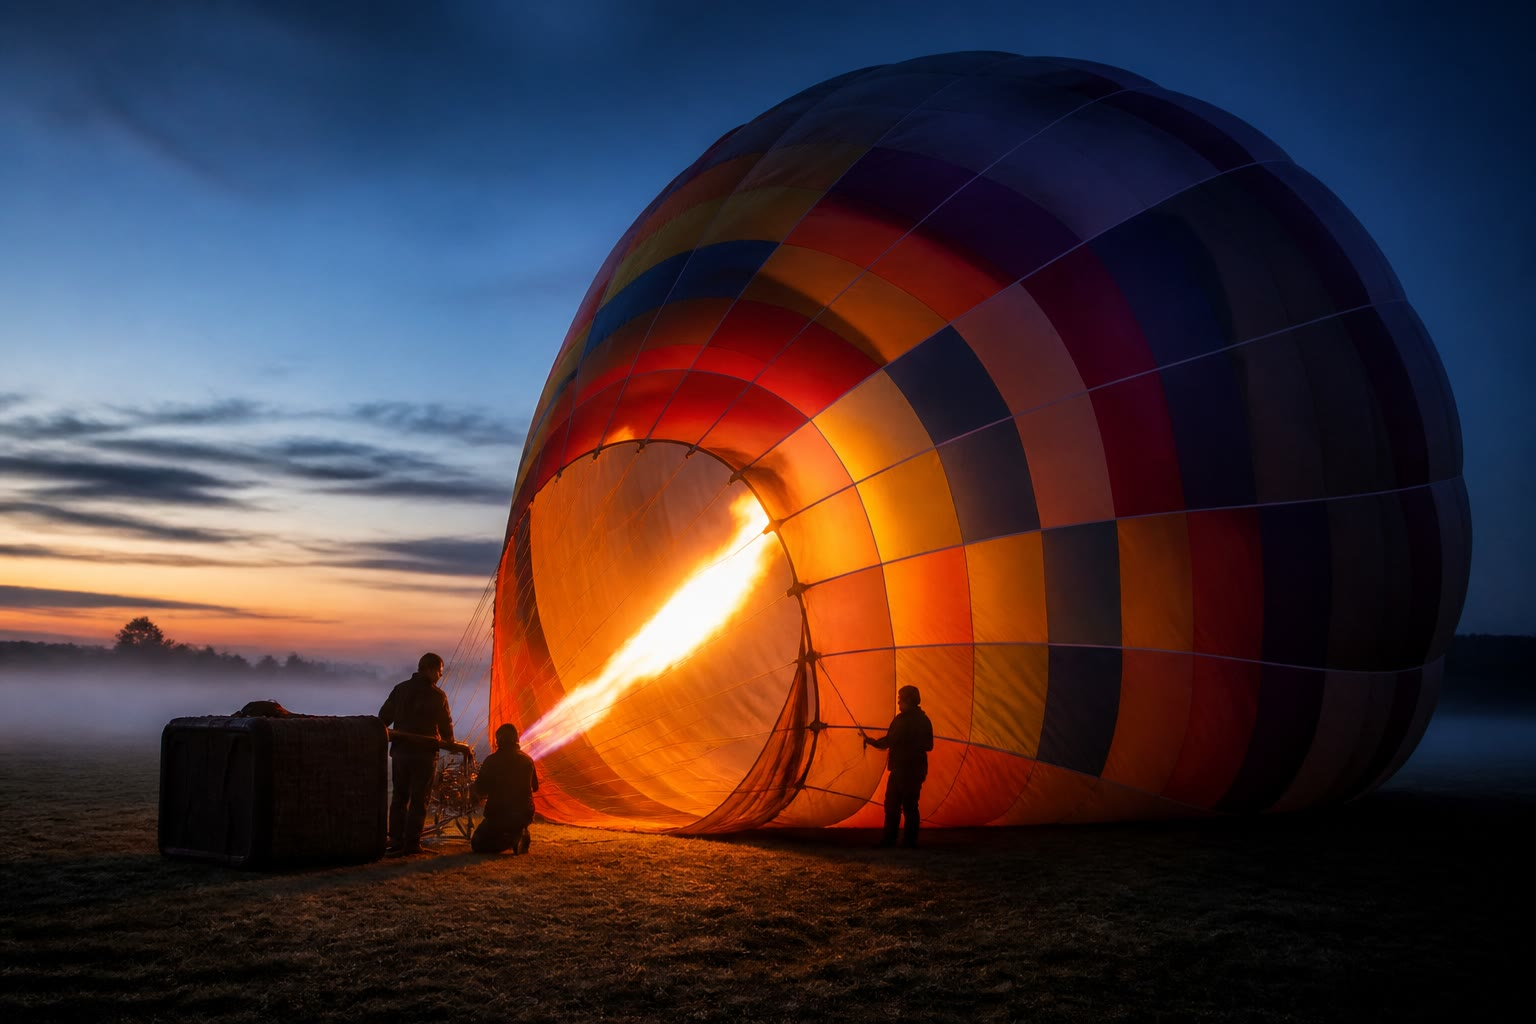
\includegraphics[width=0.58\linewidth]{images/book3/ai/b3-20-hot-air-balloon-burner.jpg}

{\small 给热气球充气：受热空气的密度小于周围冷空气，阿基米德作用于球囊上的推力超过其重力。}
\end{omfigure}

\section{问题：潜艇}

\begin{problem}[{周末问题——钢制艇体位于水下三百米处：
艇壳上的压力，为下沉而吸入、为上浮而排出的水，
离艇的潜水员，以及从其头顶经过的
油轮}]
\label{pb:b1:fluid-statics:1}
海水：$\rho = \qty{1025}{kg/m^3}$；淡水 \qty{1000}{kg/m^3}；
$P_0 = \qty{1.013e5}{Pa}$；$g = \qty{9.81}{m/s^2}$。潜艇的艇体
所围体积为 $V = \qty{3000}{m^3}$；压载舱为空时，其质量为
$m_0 = \qty{2800}{t}$。

\medskip
\noindent\textbf{第一部分——艇体上的压强。}
\begin{enumerate}
  \item 深度 \qty{300}{m} 处的绝对压强，分别以帕斯卡和巴表示。
  \item 直径为 \qty{0.80}{m} 的圆形舱口在该深度所受的力，
        与一辆卡车的重力相比较。
  \item 若艇体高 \qty{10}{m}、顶部位于 \qty{300}{m} 深处，则艇底处每平方米
        艇壳所受的力为多少？它与顶部处相比
        有何不同？
  \item 水的可压缩性很小（$\chi_T = \qty{4.6e-10}{Pa^{-1}}$），
        海水在 \qty{300}{m} 深处的密度比水面处相对增大了多少？
        这对上面算出的压强有影响吗？
  \item 艇内乘员呼吸 \qty{1}{atm} 的空气：艇壳为何须是厚壁圆柱体，
        圆柱体为何比平板箱更能抵抗压力？
        请说明理由。
  \item 半径为 $R$、壁厚为 $e$ 的薄圆柱壳，
        在外部超压 $\Delta P$ 作用下，壁内承受压应力，
        其值为 $\Delta P\,R/e$。取 $R = \qty{5.0}{m}$ 且
        $e = \qty{3.0}{cm}$，在 \qty{300}{m} 深处算出该应力，
        并与钢材约 \qty{600}{MPa} 的屈服应力相比较。
\end{enumerate}

\medskip
\noindent\textbf{第二部分——下沉与上浮。}
\begin{enumerate}[resume]
  \item 压载舱为空、位于水面时，有多大体积的艇体露出水面？
  \item 为使潜艇达到悬浮状态（中性浮力），压载舱须吸入
        多少质量的海水？
  \item 在 \qty{300}{m} 深处达到中性浮力后，艇体受压缩
        而缩小了 $0.1\%$。求由此产生的合力，并说明
        该平衡相对于深度是否稳定。
  \item 保持中性浮力的艇从海水驶入淡水河口。
        其所受合力为多少？它将朝哪个方向运动，
        艇上乘员须做什么？
  \item 一枚 \qty{20}{t} 的鱼雷被发射。压载系统须立即作何调节，
        调节量为多少？
  \item 潜艇为何用压缩空气排空压载舱，
        而空气的压强为何限制了其排水的最大深度？
  \item 估算排空 \qty{300}{m} 深处 \qty{275}{m^3} 压载舱所需的
        \qty{1}{atm} 空气体积（应用玻意耳定律，$PV$
        为常量）。
\end{enumerate}

\medskip
\noindent\textbf{第三部分——潜水员。}
一名潜水员从水面下潜，肺中含有 \qty{6.0}{L} 的空气。
\begin{enumerate}[resume]
  \item 深度 \qty{10}{m} 与 \qty{30}{m} 处的绝对压强。
  \item 若她屏住呼吸下潜，
        则在 \qty{30}{m} 深处其肺容积为多少？
  \item 一名水肺潜水员在 \qty{30}{m} 深处呼吸与环境压强相等的空气，
        若其屏住呼吸上浮，则其肺在水面处需要多大容积，
        并由此得出什么结论？
  \item 一根长 \qty{1.0}{m} 的呼吸管：潜水员胸部水压与肺内空气压强之差，
        作用在面积为 \qty{0.05}{m^2} 的胸部上的力，
        她能否吸气？
  \item 气瓶内为 \qty{200}{bar} 下的 \qty{12}{L} 空气：折合为
        \qty{30}{m} 深处的空气有多少升，并按每分钟 \qty{20}{L} 计，
        可供使用多长时间？
\end{enumerate}

\medskip
\noindent\textbf{第四部分——头顶的油轮。}
\begin{enumerate}[resume]
  \item 一艘质量为 \qty{100000}{t} 的油轮漂浮于海水中，
        求其排开海水的体积。
  \item 其水线面积为 \qty{8000}{m^2}，驶入淡水时
        船体将上浮或下沉多少？
  \item 装载 \qty{10000}{t} 石油，求吃水的变化量。
  \item 空载油轮的质心较高，故空载时以海水作压载物。
        试从稳心的角度说明其理由。
  \item 油轮龙骨处（吃水 \qty{20}{m}）的船体压强，
        及其每平方米所受的力，
        与 \qty{300}{m} 深处的潜艇作比较。
  \item 油轮恰好从潜艇正上方经过，潜艇能否感受到
        油轮 \qty{100000}{t} 的重量？
        试借助压强场加以解释。
  \item 试总结：决定本题全部数值的那一个关系式，
        以及由其导出的那条定理。
\end{enumerate}
\end{problem}
